\documentclass[11pt,twoside,a4paper]{article}
% http://www-h.eng.cam.ac.uk/help/tpl/textprocessing/latex_maths+pix/node6.html symboles de math
% http://fr.wikibooks.org/wiki/Programmation_LaTeX Programmation latex (wikibook)
%=========================== En-Tete =================================
%--- Insertion de paquetages (optionnel) ---
\usepackage[english]{babel}  % pour dire que le texte est en anglais
\usepackage{a4}	             % pour la taille   
\usepackage[T1]{fontenc}     % pour les font postscript
\usepackage{epsfig}          % pour gerer les images
\usepackage{amsmath, amsthm} % tres bon mode mathematique
\usepackage{amsfonts,amssymb}% permet la definition des ensembles
\usepackage{float}           % pour le placement des figure
\usepackage{verbatim}

%% compile with : pdflatex document.tex && pdflatex document.tex && rm *.aux *.log
\usepackage{caption}

\usepackage{longtable} % pour les tableaux de plusieurs pages

\usepackage[table]{xcolor} % couleur de fond des cellules de tableaux

\usepackage{lastpage}

% \usepackage[top=1.5cm, bottom=1.5cm, left=1.5cm, right=1.5cm]{geometry}
% gauche, haut, droite, bas, entete, ente2txt, pied, txt2pied
\usepackage{vmargin}
\setmarginsrb{1.0cm}{1.0cm}{1.0cm}{1.0cm}{15pt}{3pt}{57pt}{20pt}

\usepackage{lscape} % changement orientation page
%\usepackage{frbib} % enlever pour obtenir references en anglais
% --- style de page (pour les en-tete) ---
\pagestyle{headings}

% % % en-tete et pieds de page configurables : fancyhdr.sty

% http://www.trustonme.net/didactels/250.html

% http://ww3.ac-poitiers.fr/math/tex/pratique/entete/entete.htm
% http://www.ctan.org/tex-archive/macros/latex/contrib/fancyhdr/fancyhdr.pdf
\def\fancyTitle{Les onzes nations américaines. }
\usepackage{fancyhdr}
\pagestyle{fancy}
% \newcommand{\chaptermark}[1]{\markboth{#1}{}}
% \newcommand{\sectionmark}[1]{\markright{\thesection\ #1}}
\fancyhf{}
\fancyhead[LE,RO]{\bfseries\thepage}
\fancyhead[LO]{\bfseries\rightmark}
\fancyhead[RE]{\bfseries\leftmark}
\fancyfoot[LE]{\thepage /\pageref{LastPage} \hfill
	CREATURES -- Artificial Life, Autonomous Agents and Gaming Environment 
\hfill ... }
\fancyfoot[RO]{... \hfill
	CREATURES -- Artificial Life, Autonomous Agents and Gaming Environment 
\hfill \thepage /\pageref{LastPage}}
\renewcommand{\headrulewidth}{0.5pt}
\renewcommand{\footrulewidth}{0.5pt}
\addtolength{\headheight}{0.5pt}
\fancypagestyle{plain}{
	\fancyhead{}
	\renewcommand{\headrulewidth}{0pt}
}

%% \pagestyle{empty}

\renewcommand{\headrulewidth}{0.25pt}
\renewcommand{\footrulewidth}{0.5pt}
%% \setlength{\headheight}{85pt}
% \addtolength{\headheight}{0.5pt}
% \fancypagestyle{plain}{
% 	\fancyhead{}
% 	\fancyfoot{}
% 	\renewcommand{\headrulewidth}{0pt}
% }

%--- Definitions de nouvelles commandes ---
\newcommand{\N}{\mathbb{N}} % les entiers naturels

%============================= Corps =================================
\begin{document}

{\huge Non Article| March 01 2000~\newline CREATURES -- Artificial Life, Autonomous Agents and Gaming Environment}~\\
{\large Adamatzky, Andrew}

CREATURES -- Artificial Life, Autonomous Agents and Gaming Environment Creatures$^{TM}$ CyberLife Technology Ltd and Millennium Interactive Ltd 1996

Creatures 2$^{TM}$ CyberLife Technology Ltd and Mindscape, Inc. 1998~\\
\textbf{Keywords Cybernetics, Software, Systems}~\\

\textbf{Abstract} Reviews current software in the fields of systems and cybernetics. Contains a report on: CREATURES -- Artificial Life, Autonomous Agents and Gaming Environment which considers: morphology; nervous systems;metabolism; genetics; Albia the world; development tools; agency and multi-agency; agents for entertainment; discussion on popularity and future versions.

A field of virtual worlds, inhabited by imaginary creatures, emerged at the edge of artificial intelligence, autonomous and multi-agent systems and artificial life. This domain incorporates animating the structure and behaviour of physical worlds, interaction with users, cognitive modelling, agent architecture and language processing and solutions to many other problems. We can speculate that the field is rooted in the first autonomous mobile creature by Grey Walter (1950), Holland and Walter (1997) and the pioneer project Eliza by Weizenbaum (1966) and grown to the Oz project (Bates, 1991, 1992), spatial economics and artificial societies (Epstein and Axtell, 1996) and virtual humans(Musse et al., 1999).

Here we discuss a complete artificial life packet for PC, which incorporates state-of-the art techniques of simulation and representation of real and virtual worlds including artificial biochemistry, digital genetics, adaptive nervous systems and virtual emotions. This artificial world -- CREATURES, created by Steve Grand (1997a,b) and developed by Cambridge-based company CyberLife,gained world-wide popularity immediately since the first release on the market. However, we are interested in this product not because of its business success but because it gives a first ever example of commercial software, which combines up-to-date achievements of natural and engineering sciences, top-down design,the reductionism view on nature and orientation, to the general audience.

Albia, cyber-world of CREATURES, is inhabited by Norns, species of virtual creatures. Norns have their own reduced anatomy and life-like biochemistry. They can mate with each other and transfer genetic information via digital DNA. Every Norn starts its life when it hatches from an egg. It matures and becomes older during its life span. Norns' behaviour is driven by a combination of external, e.g. user defined stimuli, and internal, e.g. changes in chemical concentrations or neural activities, events. Norns possess intrinsic interest for exploration, appealing to everyone's emotions and hidden desires;they are good learners but make mistakes.

\textbf{Morphology}~\\

Creature morphology is primitive (Figure 1)~\footnote{All screenshots, illustrating the review, are made from CREATURES$^TM$ -- the first release of software.}. No visceral organs are designed, neither bones nor muscles. Based on sprite representation we counted about 14 body parts of Norn. They include head, body, thighs, shins, feet and tails. Unreasonably, muscles are classified as chemicals. Luckily the absence of proper models of organs is substituted by concepts of the organs as subjects of influence or causes of influence, concepts which produce or consume chemicals. Therefore, we can monitor the activity of imaginary muscles, lungs, liver,biological clocks, bones, skin, sex hormone glands, uterus.

\clearpage

\begin{minipage}[ht]{0.45\textwidth}
	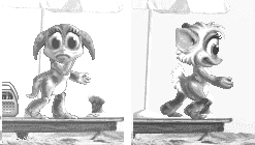
\includegraphics[width=0.90\textwidth]{m_k_2000_06729bad_001-1v29b001.png}
	\captionof{figure}{Front and side views of Norn the creature}
	\label{fig:nornviews}
\end{minipage} \hfill \begin{minipage}[ht]{0.45\textwidth}	
	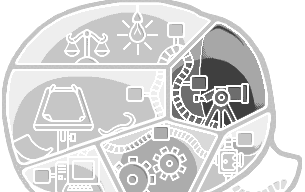
\includegraphics[width=0.90\textwidth]{m_k_2000_06729bad_001-1v29b002.png}
	\captionof{figure}{Compartments of the Norn brain. Vision related lobe is activated}
	\label{fig:nornbraincomparment}
\end{minipage}~\\

\textbf{Nervous system}~\\

It is claimed that the Norn brain consists of almost 1,000 neurones; however,we could not check it without knowing the code. All we know for sure is that the brain is built up of ten "lobes" (Figure 2): perception lobe, drive lobe,stimulation sources lobe, verb lobe, noun lobe, general sense lobe, decision lobe, attention lobe, concept lobe and regular lobe. Sensory inputs activate a general sense lobe and a stimulation sources lobe. Activity of the general sense lobe is integrated with activity of the drive lobe and verb lobe. They subsequently activate perceptible senses, sensory schemata and action schemata. As a result an action output is formed. The stimulation sources lobe is integrated with the noun lobe and activates the attention lobe. Thus, a focus of attention is made up. There is also a one-way connection from attention to perceptible senses. Such a general anatomy of the creature's brain supports a current of nervous activity along the cycle "stimulus -> concept ->action".~\\

The vocational abilities of Norns are satisfactory and based on a vocabulary of up to 80 words. Ideally, each creature is completely individual, has its own personality and behavioural patterns. This is because individual creatures are not explicitly programmed. However, practically, it may be difficult to differentiate between two creatures without certain experience.~\\

\textbf{Metabolism}~\\

The metabolic paths of the creatures are quite correct even taking into account that a lot of fictional chemicals, or would-be chemicals, are used,which actually generalise several real chemicals in one. Among 250 chemicals,several groups can be selected:

\begin{itemize}
	\item Fictional abstract chemicals responsible for pain level, need for pleasure,hunger, sleepiness, crowding, anger, sex drive, dancing. There are also drive raising and drive reducing substances.
	\item Chemicals used in learning, e.g. reinforcement, reward, and punishment. The class includes such exotic substances as the atrophy reinforcement hormone of the concept layer and the decision layer of the Norn brain.
	\item Components with real names, e.g. triglyceride, some amino acids, carbon dioxide, progesterone, cholesterol, anabolic steroids, heavy metals, and belladonna.
	\item Pheromones, e.g. mating, species, child etc. pheromones.
	\item Vitamins.
	\item Antigens and antibodies.
\end{itemize}

The choice of chemicals is quite arbitrary; however, it does not contradict to a common sense. It rather reflects an uneducated view on inorganic chemistry and biochemistry, which may pleasantly appeal to the educational background of an average user. The integral dynamic of interacting chemicals correctly fits the graphs produced by a system of differential equations (Figure 3). Thus no arguments against the generalisation approach to metabolism can be found.

\begin{minipage}[ht]{0.45\textwidth}
		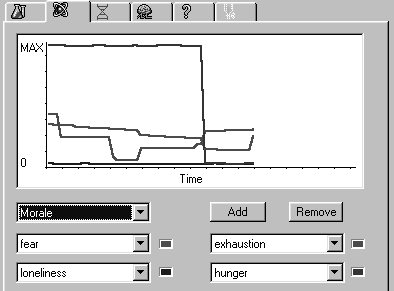
\includegraphics[width=0.90\textwidth]{m_k_2000_06729bad_001-1v29b003.png}
		\captionof{figure}{Monitoring metabolism}
		\label{fig:monitoringmetabolism}
\end{minipage} \hfill \begin{minipage}[ht]{0.45\textwidth}	
		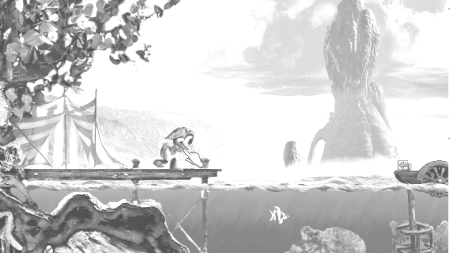
\includegraphics[width=0.90\textwidth]{m_k_2000_06729bad_001-1v29b004.png}
		\captionof{figure}{Snapshot of the CREATURES world}
		\label{fig:snapshotCREATURESworld}
\end{minipage}~\\

\textbf{Genetics}~\\

A quite sophisticated form of information transfer from parents to offspring is provided in the model via a concept of digital DNA. The digital DNA has nothing to do with real DNA except in association. However, complete information about creatures is coded in genes. There are almost 800 Norn genes in CREATURES 2. Half of all genes are responsible for behavioural patterns and physical appearance while the other half are involved in determination of biochemistry and the nervous system.

Following their concept of digital DNA the creators supplied every gene with a header. The header of a gene stores information about the range of possible operations on the gene: duplication, mutation and deletion. This prevents occurrence of a catastrophic situation when vital genes are deleted and the population is put under threat of extinction.

Creature diversity is reached because of cross-over, which happens when chromosomes replicate. At this stage, a mixture of genes from both parents is produced. Sometimes several "organs" are generated or some organs are missed. The accidents with redundancy or lack of organs do not influence the creatures'life in general because there is no proper anatomy or physiology. Sex determined gene expressions are employed in creature genetics.

For an advanced user a special tool -- genetics editor -- is supplied. The tool allows the user to change phenotypes by linking certain genes to new designs of body parts. Pigmentation and instincts are the most expressive criteria for potential selection.

\textbf{Albia the world}~\\
	
A room is a basic unit of CREATURES world. There are four types of rooms: indoors, surface, underwater and atmosphere (Figure 4). The authors claim that the physics of every room is represented in a cellular-automata model,where parameters are changed locally but with global consequences. This would be reasonable; however, we did not find any proofs of such cellular-automata representation. A list of room properties includes pressure, temperature,illumination, radiation and concentrations of organic and inorganic nutrients. To control movement and interactions of in-game objects the ecology kit is used. The chemicals may be injected with the help of a chemical mixing machine.

\textbf{Development tools}~\\

Using OLE interface you can set up communication with CREATURES software from any external program written on a common programming language. Moreover, you can design new agents and implement them in CAOS scripting language and inject them in the virtual worlds after that. Every agent is represented in a special Creature Object format. The objects are classified as a creature, a simple object (e.g. physical object, elementary unit) which has boundaries and is mobile, compound object (physical object of many parts) which may include other objects inside it, and scenery item, which consists of non-physical objects (i.e. some background). Further classification allows specifying how the objects behave and how they are used.~\\

\textbf{Agency and multi-agency}~\\

Minimal autonomous agents have goals and needs, perception of an environment and competition of needs; also they can act. Sensing and acting are quite explicit in CREATURES. A goal-oriented component is not so pellucid. Generally, Norns do not have goals. They even do not want to stay alive. However, absence of long-term goals makes CREATURES advantageous in comparison with other intelligent games. No predetermined patterns of Norn behaviour, except probably basic ones, are incorporated in creature architecture. Current goals can be chosen and lost very fast in real time. Thus Norn behaviour becomes adaptive up to a certain degree.~\\

It is worth indicating the position of Norns in the hierarchy of adaptive agents. One of the recent taxonomies (Nareyek, 2000) includes reactive agents(they follow if-then rules), triggering agents (they have internal states and attain long-term tasks), deliberative agents (they have internal planning system), hybrid agents and anytime agents (provide a continuum from reaction to planning). Norns are classified as triggering agents (Nareyek, 2000) because they can form several internal concepts at a time; the concepts determine range of creature reaction on external stimuli. The neural network makes creatures learning from real-time changes in their environment. From the hierarchy we see that Norns are on the second step of the adaptive agent evolution ladder.~\\

CREATURES set-up does not pass the test on multi-agency. Depending on the particular version of CREATURES the virtual world can not accept more than eight to 12 intelligent agents. Creatures can play with, like or dislike each other, and mate with one another. However, they are unable to solve a problem at a distributive level. No proper collective actions are observed and no decentralised or distributed knowledge is detected.~\\

\textbf{Agents for entertainment}~\\

Autonomy is a main feature of artificial living entities. How long could Norns live without user invention? Surprisingly, not as long as necessary. They are very dependent on their human masters. Hence such dependence invokes a feeling of responsibility in players. The creatures are personalizable. Norns maintain their own personality of responses on external events. They have a programmable lexicon and they are also capable of recording information accessible from other sources. Co-operation is a difficult matter when talking about Norns. They are not co-operative. Creatures do not collaborate with the players or with other inhabitants of Albia. Even some kind of reduced two-way co-operation between player and creatures does not improve their capabilities to be team players.~\\

CREATURES game environment uses classical techniques for displaying a character in such a manner as to invoke the desired emotional response from the player. They include physical reactions, context of emotions, sound and scenery. All actors must be robust. They should not do anything which may underpin a player's belief in the actor reality (Reilly, 1996), i.e. the agents must react as intelligent entities. Not all program realisations allow the enrichment of actors with intelligence. In most cases agent dumbness is concealed. In CREATURESintellectually handicapped agents behave like children. That is, an impression is made that Norns understand everything you want but they do not want to do it:~\\

Choosing personality traits that allow for believable unresponsiveness can make the characters easier to build and more effective than characters that should be responsive but aren't (Reilly, 1996).~\\

In this way the user expectations are lowered and a range of possible interactions between user and actor and among actors themselves is narrowed down~\\

Regarding the communicating abilities of creatures we should mention a couple of similar, up to some degree, chatterboxes developed recently. The first of them is built on the result of the Persona project conducted at Microsoft Research. A life-like animated character for interacting with users in natural languages -- Peedy the Parrot -- a three-dimensional anthropomorphic personage,who responds to user requests on music (Ball et al., 1997). The second is an animation and chat engine -- Virtual Friend -- designed at Haptek Inc. (2000). It displays realistic three-dimensional characters with whom the user interacts in real time. The characters express emotions, react to user-induced events, can speak to you and teach you. The user can tune his friend's voice, change the background and texture. More than 60 friends can be downloaded and played with. In these two examples we can gain much intellectual communication but will suffer the absence of the real world environment; also no reproduction is allowed.~\\

\clearpage

\textbf{Why are they so popular?}~\\

Since the launch of the product hundreds of thousands of copies have been sold all over the world and the number of users grows exponentially. The success of any software product is a very mystical and unknowable feature. Subtle trends and emergent properties of the market determine it. However, few obvious reasons can be cited here. The first one is attitude. The entire system is done with care and with orientation to a wide audience:

Something a naturalist would want to study, a father would want to teach soccer, a granny to dress up and a complete b***ard to butcher mercilessly...(CREATURES, 2000).

Naiveté is the second feature. A balance between simplicity and complexity is kept at all levels of system environment and development tools. The success of the reductionistic approach is clear. The creatures are

...human enough to have recognisable facial expressions yet animal enough to be kept as a pet ...(CREATURES, 2000).

The system is open. This is the third feature. The artificial world and all its inhabitants can be modified; users themselves can design new components. CyberLife Technology Ltd actively interacts with the users via Creature Developer Network, a technical forum of CREATURES users. A world community of CREATURES users is generated; somewhere artificially by CyberLife Technology Ltd, somewhere naturally by users themselves. Thus, for example, a moderated list for technical discussions related to the CREATURESproduct is founded under the name of \emph{The Journal of Albian Ecology} (2000). The "Backstreet of Albia" section of CyberLife Technology Web site also appeals to emotional fans of CREATURES. There everyone can find fiction,cartoons and poems written by users about creatures and on behalf of creatures. A \emph{mysticism} of CREATURES world is the last but not the least feature. This is made by the appearance of gremlins, phonetics as in Klingon language and the environment of Wookey Hole. As a Norn may say:~\\

Neither the world nor I have physical form, but we do exist, and I am alive...(CREATURES 2000).~\\

\textbf{What next?}~\\

As recently announced, the third version of CREATURES is on its way to the public. The CREATURES 3 world will include several terraria with their own ecosystems, food chains, climate and seasonal changes. The terraria will be inhabited by intelligent creatures of three species accompanied by a wide range of animals and plants. Moreover, the "traditional" CREATURESenvironment is adapted now for a young audience in CREATURES ADVENTURErecently released on the market. The product features simplified interface,stimulation for playing and explorations, and a rich range of interactions with objects.~\\

\clearpage

\textbf{Bibliograpgy}~\\

Andrew Adamatzky \emph{Intelligent Autonomous Systems Lab, University of the West of England, Bristol, UK}

CREATURES, "History", \texttt{http://www.creatures.co.uk/Library/lib\_history.htm}~\\

Epstein, J.M. and Axtell, R.L. (1996), \emph{Growing Artificial Societies}, The MIT Press.

Grand, S. (1997a), "Creatures: an exercise in creation", IEEE Expert.

Grand, S., Cliff, D. and Malhorta, A. (1997b), "Creatures: artificial life,autonomous software agents for home entertainment", Proc. 1st Int. Conf. on Autonomous Agents, ACM Press, New York, NY, pp. 22-9.

Haptek$^{TM}$ Inc., http://www.haptek.com

Holland, O. and Walter, G. (1997), "The pioneer of real artificial life", Artificial Life V, The MIT Press, pp. 34-41.

Musse, S.R., Kallmann, M. and Thalmann, D. (1999), "Level of autonomy for virtual human agents", Advances in Artificial Life, Springer, pp. 345-9.

Nareyek, A. (2000), "Excalibur: adaptive constraint-based agents in artificial environments, 1997-1999", Project homepage: http://www.first.gmd.de/concorde/excaliburhome.html

Reilly, S.W. (1996), "Believable social and emotional agents", Technical Report CMU-CS-96-138, Carnegie Mellon School of Computer Science.

\emph{The Journal of Albian Ecology}, \texttt{http://journalbecol.listbot.com}

Walter, G. (1950), "An imitation of life", Scientific American, pp. 42-5.

Weizenbaum, J.E. (1966), "A computer program for the study of natural language communication between man and machine", Communications ACM 9,pp. 36-45.

\textbf{References}~\\

Ball, G., Ling, D., Kurlander, D., Miller J. et al. (1997), "Lifelike computer characters: the Persona project at Microsoft Research", http://www.research.microsoft.com/research/ui/persona/chapter/persona.htm

Bates, J. (1991), "Deep structure for virtual reality", Technical Report CMU-CS-91-133, Carnegie Mellon School of Computer Science.

Bates, J. (1992), "The nature of character in interactive worlds and the Oz project", Technical Report CMU-CS-92-200, Carnegie Mellon School of Computer Science.



\end{document}
